\section{Results} \label{sec:results}
This section presents the numerical results obtained by the proposed methods. To better compare the numerical results, Table \ref{tab:expected} shows the expected integration values for each function.
\begin{table}[H]
    \centering
    \caption{Expected Integration Values.}
    \label{tab:expected}
    \begin{tabular}{ccccc}
    \hline
    \textbf{Function}  & \makecell{1 \\ ($\epsilon = 1$)} & \makecell{1 \\ $\left(\epsilon = 10^{-4}\right)$} & 2 & 3 \\ 
    \textbf{Expected Value} & 1.49364 & 0.01772 & -0.00089 & 11.63905 \\ \hline
    \end{tabular}
\end{table}

Tables \ref{tab:trapezoidal_int} - \ref{tab:gauss4_rate} show the numerical integration and rate of convergence for all three functions, using the four integration rules. 



\begin{table}[H]
    \centering
    \caption{Trapezoidal Rule: Numerical Integration.}
    \label{tab:trapezoidal_int}
    \begin{tabular}{ccc|ccc}
    \hline
    \multicolumn{3}{c}{\textbf{Function 1  -} $\bm{\epsilon = 1}$} & \multicolumn{3}{c}{\textbf{Function 1 -} $\bm{\epsilon = 10^{-4}}$} \\ \hline
    N. Intervals & Approx. Sol. & $|| e ||$ & N. Intervals & Approx. Sol. & $|| e ||$ \\ \hline
    1 & 0.73575 & 0.75788 & 1 & 0.0 & 0.01772 \\
    2 & 1.36787 & 0.12576 & 2 & 1.0 & 0.98227 \\
    4 & 1.46274 & 0.03541 & 4 & 0.5 & 0.48227 \\
    8 & 1.48596 & 0.010195 & 8 & 0.25 & 0.23227 \\
    16 & 1.49173 & 0.00253 & 16 & 0.125 & 0.10727 \\
    32 & 1.49316 & 0.00063 & 32 & 0.0625 & 0.04477 \\ \hline
    \multicolumn{3}{c}{\textbf{Function 2}} & \multicolumn{3}{c}{\bf{Function 3}} \\ \hline
    N. Intervals & Approx. Sol. & $|| e ||$ & N. Intervals & Approx. Sol. & $|| e ||$ \\ \hline
    1 &  {-0.00267} &  {0.00177} & 1 &  {9.42822} &  {2.21083} \\
    2 &  {-0.00287} &  {0.00197} & 2 &  {11.56799} &  {1.5334} \\
    4 &  {-0.00129} &  {0.00243} & 4 &  {11.62885} &  {0.34341} \\
    8 &  {-0.00154} &  {0.00173} & 8 &  {11.63645} &  {0.09581} \\
    16 &  {-0.00087} &  {0.00064} & 16 &  {11.63840} &  {0.02383} \\
    32 &  {-0.00092} &  {0.00039} & 32 &  {11.63889} &  {0.00595} \\ \hline
    \end{tabular}
\end{table}
\begin{table}[H]
    \centering
    \caption{Trapezoidal Rule: Rate of Convergence.}
    \label{tab:trapezoidal_rate}
    \begin{tabular}{ccccccc}
        \hline
        \multirow{2}{*}{\textbf{Function}} & \multicolumn{5}{c}{\textbf{Subintervals}} & \multicolumn{1}{c}{\multirow{2}{*}{\textbf{Average Rate}}} \\ \cline{2-6}
 & (1 - 2) & (2 - 4) & (4 - 8) & (8 - 16) & (16 - 32) & \multicolumn{1}{c}{} \\ \hline
        \makecell{1 \\ ($\epsilon = 1$)} & -2.59 & -1.83 & -1.80 & -2.01 & -1.99 & -2.04 \\
        \makecell{1 \\ $\left(\epsilon = 10^{-4}\right)$} & 5.79 & -1.03 & -1.05 & -1.11 & -1.26 & 0.27 \\
        2 & 0.15 & 0.31 & -0.49 & -1.42 & -0.72 & -0.43 \\ 
        3 & -0.53 & -2.16 & -1.84 & -2.01 & -2.00 & -1.71 \\ \hline
    \end{tabular}
\end{table}

\begin{table}[H]
    \centering
    \caption{Simpson 1/3 Rule: Numerical Integration.}
    \label{tab:simpson13_int}
    \begin{tabular}{ccc|ccc}
    \hline
    \multicolumn{3}{c}{\textbf{Function 1  -} $\bm{\epsilon = 1}$} & \multicolumn{3}{c}{\textbf{Function 1 -} $\bm{\epsilon = 10^{-4}}$} \\ \hline
    N. Intervals & Approx. Sol. & $|| e ||$ & N. Intervals & Approx. Sol. & $|| e ||$ \\ \hline
    1 & 1.57858 & 0.08493 & 1 & 1.33333& 1.31560 \\
    2 & 1.49436 & 0.00071 & 2 & 0.33333 & 0.31560 \\
    4 & 1.49371 & 0.00029 & 4 & 0.16666 & 0.14894 \\
    8 & 1.49365 & 1.74e-05 & 8 & 0.08333 & 0.06560 \\
    16 & 1.49364 & 1.07e-06 & 16 & 0.04166 & 0.02394 \\
    32 & 1.49364 & 6.70e-08 & 32 & 0.02083 & 0.00311 \\ \hline
    \multicolumn{3}{c}{\textbf{Function 2}} & \multicolumn{3}{c}{\bf{Function 3}} \\ \hline
    N. Intervals & Approx. Sol. & $|| e ||$ & N. Intervals & Approx. Sol. & $|| e ||$ \\ \hline
    1 & -0.00293  & 0.00203  & 1 & 12.28124 &  0.64219 \\
    2 & -0.00077  & 0.00210  & 2 & 11.64914 &  0.05324 \\
    4 & -0.00162  & 0.00113  & 4 & 11.63898  & 0.00222 \\
    8 & -0.00064 & 0.00059  & 8 &  11.63905 &  0.00015 \\
    16 & -0.00094 & 0.00021 & 16 & 11.63905 &  9.52e-06 \\
    32 & -0.00082 & 8.50e-05  & 32 & 11.63905  & 5.93e-07  \\ \hline
    \end{tabular}
\end{table}
\begin{table}[H]
    \centering
    \caption{Simpson 1/3 Rule: Rate of Convergence.}
    \label{tab:simpson13_rate}
    \begin{tabular}{ccccccc}
        \hline
        \multirow{2}{*}{\textbf{Function}} & \multicolumn{5}{c}{\textbf{Subintervals}} & \multicolumn{1}{c}{\multirow{2}{*}{\textbf{Average Rate}}} \\ \cline{2-6}
 & (1 - 2) & (2 - 4) & (4 - 8) & (8 - 16) & (16 - 32) & \multicolumn{1}{c}{} \\ \hline
        \makecell{1 \\ ($\epsilon = 1$)} & -6.90 & -1.26 & -4.09 & -4.02 & -4.01 & -4.05 \\
        \makecell{1 \\ $\left(\epsilon = 10^{-4}\right)$} & -2.06 & -1.08 & -1.18 & -1.45 & -2.94 & -1.74 \\
        2 & 0.05 & -0.89 & -0.92 & -1.50 & -1.32 & -0.92 \\ 
        3 & -3.59 & -4.58 & -3.86 & -4.01 & -4.00 & -4.01 \\ \hline
    \end{tabular}
\end{table}

\begin{table}[H]
    \centering
    \caption{Simpson 3/8 Rule: Numerical Integration.}
    \label{tab:simpson38_int}
    \begin{tabular}{ccc|ccc}
    \hline
    \multicolumn{3}{c}{\textbf{Function 1  -} $\bm{\epsilon = 1}$} & \multicolumn{3}{c}{\textbf{Function 1 -} $\bm{\epsilon = 10^{-4}}$} \\ \hline
    N. Intervals & Approx. Sol. & $|| e ||$ & N. Intervals & Approx. Sol. & $|| e ||$ \\ \hline
    1 & 1.52619 & 0.03255 & 1 & 0.0 & 0.01772 \\
    2 & 1.49398 & 0.00033 & 2 & 0.25 & 0.23227 \\
    4 & 1.49367 & 0.00013 & 4 & 0.125 & 0.10727 \\
    8 & 1.49365 & 7.75e-06 & 8 & 0.0625 & 0.04477 \\
    16 & 1.49364 & 4.7e-07 & 16 & 0.03125 & 0.01352 \\
    32 & 1.49364 & 2.97e-08 & 32 & 0.01623 & 0.00148 \\ \hline
    \multicolumn{3}{c}{\textbf{Function 2}} & \multicolumn{3}{c}{\bf{Function 3}} \\ \hline
    N. Intervals & Approx. Sol. & $|| e ||$ & N. Intervals & Approx. Sol. & $|| e ||$ \\ \hline
    1 & 0.00148  & 0.00238 & 1 & 11.91167 & 0.27261  \\
    2 & -0.00035  & 0.00075 & 2 & 11.63937 & 0.01908  \\
    4 & -0.00065 & 0.00028 & 4 & 11.63902 & 0.00098 \\
    8 & -0.00077 & 0.00015 & 8 &  11.63905 &  6.82e-05 \\
    16 & -0.00082 & 0.00013 & 16 & 11.63905 &  4.23e-06 \\
    32 & -0.00089 & 3.67e-05  & 32 & 11.63905 & 2.63e-07  \\ \hline
    \end{tabular}
\end{table}
\begin{table}[H]
    \centering
    \caption{Simpson 3/8 Rule: Rate of Convergence.}
    \label{tab:simpson38_rate}
    \begin{tabular}{ccccccc}
        \hline
        \multirow{2}{*}{\textbf{Function}} & \multicolumn{5}{c}{\textbf{Subintervals}} & \multicolumn{1}{c}{\multirow{2}{*}{\textbf{Average Rate}}} \\ \cline{2-6}
 & (1 - 2) & (2 - 4) & (4 - 8) & (8 - 16) & (16 - 32) & \multicolumn{1}{c}{} \\ \hline
        \makecell{1 \\ ($\epsilon = 1$)} & -6.60 & -1.36 & -4.08 & -4.02 & -4.00 & -4.01 \\
        \makecell{1 \\ $\left(\epsilon = 10^{-4}\right)$} & 3.71 & -1.11 & -1.26 & -1.73 & -3.18 & -0.71 \\
        2 & -1.67 & -1.40 & -0.91 & -0.13 & -1.92 & -1.20 \\ 
        3 & -3.84 & -4.28 & -3.85 & -4.01 & -4.00 & -4.00 \\ \hline
    \end{tabular}
\end{table}

\begin{table}[H]
    \centering
    \caption{Gauss-Legendre Rule - 1 point: Numerical Integration.}
    \label{tab:gauss1_int}
    \begin{tabular}{ccc|ccc}
    \hline
    \multicolumn{3}{c}{\textbf{Function 1  -} $\bm{\epsilon = 1}$} & \multicolumn{3}{c}{\textbf{Function 1 -} $\bm{\epsilon = 10^{-4}}$} \\ \hline
    N. Intervals & Approx. Sol. & $|| e ||$ & N. Intervals & Approx. Sol. & $|| e ||$ \\ \hline
    1 & 2.0 & 0.50635 & 1 & 2.0 & 1.98227 \\
    2 & 1.5576 & 0.06395 & 2 & 0.0 & 0.01772 \\
    4 & 1.50919 & 0.01815 & 4 & 3.68e-272 & 0.01772 \\
    8 & 1.49749 & 0.00511 & 8 & 6.92e-69 & 0.01772 \\
    16 & 1.49460 & 0.00127 &  16 & 2.71e-18 & 0.01772 \\
    32 & 1.49388 & 0.00031 & 32 & 7.17e-06 & 0.01771 \\ \hline
    \multicolumn{3}{c}{\textbf{Function 2}} & \multicolumn{3}{c}{\bf{Function 3}} \\ \hline
    N. Intervals & Approx. Sol. & $|| e ||$ & N. Intervals & Approx. Sol. & $|| e ||$ \\ \hline
    1 & -0.00306 & 0.00216 & 1 & 13.70776 & 2.06870\\
    2 & 0.00027& 0.00315 & 2 & 11.68971 & 0.84657\\
    4 & -0.00178 & 0.00194 & 4 & 11.64404 & 0.17504\\
    8 & -0.00020 & 0.00163 & 8 & 11.64035 & 0.04813\\
    16 & -0.00098 & 0.00055 & 16 & 11.63938 & 0.01193\\
    32 & -0.00077 & 0.00029 & 32 & 11.63914& 0.00297 \\\hline
    \end{tabular}
\end{table}
\begin{table}[H]
    \centering
    \caption{Gauss-Legendre Rule - 1 point: Rate of Convergence.}
    \label{tab:gauss1_rate}
    \begin{tabular}{ccccccc}
        \hline
        \multirow{2}{*}{\textbf{Function}} & \multicolumn{5}{c}{\textbf{Subintervals}} & \multicolumn{1}{c}{\multirow{2}{*}{\textbf{Average Rate}}} \\ \cline{2-6}
 & (1 - 2) & (2 - 4) & (4 - 8) & (8 - 16) & (16 - 32) & \multicolumn{1}{c}{} \\ \hline
        \makecell{1 \\ ($\epsilon = 1$)} & -2.99 & -1.82 & -1.83 & -2.01 & -2.00 & -2.13 \\
        \makecell{1 \\ $\left(\epsilon = 10^{-4}\right)$} & -6.81 & 0.00 & 0.00 & 0.00 & 0.00 & -1.36 \\
        2 & 0.54 & -0.69 & -0.25 & -1.57 & -0.92 & -0.58 \\ 
        3 & -1.29 & -2.27 & -1.86 & -2.01 & -2.00 & -1.89 \\ \hline
    \end{tabular}
\end{table}

\begin{table}[H]
    \centering
    \caption{Gauss-Legendre Rule - 2 points: Numerical Integration.}
    \label{tab:gauss2_int}
    \begin{tabular}{ccc|ccc}
    \hline
    \multicolumn{3}{c}{\textbf{Function 1  -} $\bm{\epsilon = 1}$} & \multicolumn{3}{c}{\textbf{Function 1 -} $\bm{\epsilon = 10^{-4}}$} \\ \hline
    N. Intervals & Approx. Sol. & $|| e ||$ & N. Intervals & Approx. Sol. & $|| e ||$ \\ \hline
    1 & 1.43306 & 0.06058 & 1 & 0.0 & 0.01772 \\ 
    2 & 1.49318 & 0.00045 & 2 & 1.12e-194 & 0.01772 \\
    4 & 1.49360 & 0.00019 & 4 & 1.62e-49 & 0.01772 \\
    8 & 1.49364 & 1.16e-05 & 8 & 1.88e-13 & 0.01772 \\
    16 & 1.49364 & 7.17e-07 & 16 & 0.00011 & 0.01760 \\
    32 & 1.49364 & 4.46e-08 & 32 & 0.01092 & 0.00680  \\ \hline
    \multicolumn{3}{c}{\textbf{Function 2}} & \multicolumn{3}{c}{\bf{Function 3}} \\ \hline
    N. Intervals & Approx. Sol. & $|| e ||$ & N. Intervals & Approx. Sol. & $|| e ||$ \\ \hline
    1 & -0.00066 & 0.00023 & 1 & 11.14786 & 0.49119 \\
    2 & -0.00135 & 0.00099 & 2 & 11.63349 & 0.03471 \\
    4 & -0.00069 & 0.00150 & 4 & 11.63910 & 0.00148 \\
    8 & -0.00112 & 0.00023 & 8 & 11.63906 & 0.00010 \\
    16 & -0.00081 & 0.00015 & 16 & 11.63905 & 6.34e-06 \\
    32 & -0.00095 & 7.48e-05 & 32 & 11.63905 & 3.95e-07 \\ \hline
    \end{tabular}
\end{table}
\begin{table}[H]
    \centering
    \caption{Gauss-Legendre Rule - 2 points: Rate of Convergence.}
    \label{tab:gauss2_rate}
    \begin{tabular}{ccccccc}
        \hline
        \multirow{2}{*}{\textbf{Function}} & \multicolumn{5}{c}{\textbf{Subintervals}} & \multicolumn{1}{c}{\multirow{2}{*}{\textbf{Average Rate}}} \\ \cline{2-6}
 & (1 - 2) & (2 - 4) & (4 - 8) & (8 - 16) & (16 - 32) & \multicolumn{1}{c}{} \\ \hline
        \makecell{1 \\ ($\epsilon = 1$)} & -7.04 & -1.20 & -4.10 & -4.02 & -4.01 & -4.07 \\
        \makecell{1 \\ $\left(\epsilon = 10^{-4}\right)$} & 0.00 & 0.00 & 0.00 & -0.01 & -1.37 & -0.28 \\
        2 & 2.06 & 0.60 & -2.65 & -0.58 & -1.10 & -0.33 \\ 
        3 & -3.82 & -4.54 & -3.86 & -4.01 & -4.00 & -4.05 \\ \hline
    \end{tabular}
\end{table}

\begin{table}[H]
    \centering
    \caption{Gauss-Legendre Rule - 3 points: Numerical Integration.}
    \label{tab:gauss3_int}
    \begin{tabular}{ccc|ccc}
    \hline
    \multicolumn{3}{c}{\textbf{Function 1  -} $\bm{\epsilon = 1}$} & \multicolumn{3}{c}{\textbf{Function 1 -} $\bm{\epsilon = 10^{-4}}$} \\ \hline
    N. Intervals & Approx. Sol. & $|| e ||$ & N. Intervals & Approx. Sol. & $|| e ||$ \\ \hline
    1 & 1.49867 & 0.00503 & 1 & 0.88888 & 0.87116 \\
    2 & 1.49362 & 1.90e-05 & 2 & 3.82e-56 & 0.01772 \\
    4 & 1.49364 & 1.16e-06 & 4 & 4.49e-15 & 0.01772 \\
    8 & 1.49364 & 1.66e-08 & 8 & 4.95e-05 & 0.01767 \\
    16 & 1.49364 & 2.55e-10 & 16 & 0.00954 & 0.00818  \\
    32 & 1.49364 & 4.05e-12 & 32 & 0.02114 & 0.00341 \\ \hline
    \multicolumn{3}{c}{\textbf{Function 2}} & \multicolumn{3}{c}{\bf{Function 3}} \\ \hline
    N. Intervals & Approx. Sol. & $|| e ||$ & N. Intervals & Approx. Sol. & $|| e ||$ \\ \hline
    1 & -0.00388 & 0.00298 & 1 & 11.66141&  0.02235 \\
    2 & -0.00104 & 0.00015 & 2 & 11.64364 & 0.00499 \\
    4 & -0.00120 & 0.00051 & 4 & 11.63905 & 5.18e-06 \\ 
    8 & -0.00079 & 0.00012 & 8 & 11.63905 & 8.91e-08 \\
    16 & -0.00099 & 0.00010 & 16 & 11.63905 & 1.37e-09 \\ 
    32 & -0.00087 & 4.45e-05 & 32 & 11.63905 & 2.14e-11 \\ \hline
    \end{tabular}
\end{table}
\begin{table}[H]
    \centering
    \caption{Gauss-Legendre Rule - 3 points: Rate of Convergence.}
    \label{tab:gauss3_rate}
    \begin{tabular}{ccccccc}
        \hline
        \multirow{2}{*}{\textbf{Function}} & \multicolumn{5}{c}{\textbf{Subintervals}} & \multicolumn{1}{c}{\multirow{2}{*}{\textbf{Average Rate}}} \\ \cline{2-6}
 & (1 - 2) & (2 - 4) & (4 - 8) & (8 - 16) & (16 - 32) & \multicolumn{1}{c}{} \\ \hline
        \makecell{1 \\ ($\epsilon = 1$)} & -8.04 & -4.03 & -6.13 & -6.03 & -5.98 & -6.04 \\
        \makecell{1 \\ $\left(\epsilon = 10^{-4}\right)$} & -5.62 & 0.00 & 0.00 & -1.11 & -1.26 & 1.60 \\
        2 & -4.27 & 1.73 & -2.00 & -0.30 & -1.23 & -1.21 \\ 
        3 & -2.16 & -9.91 & -5.86 & -6.01 & -6.00 & -5.99 \\ \hline
    \end{tabular}
\end{table}

\begin{table}[H]
    \centering
    \caption{Gauss-Legendre Rule - 4 points: Numerical Integration.}
    \label{tab:gauss4_int}
    \begin{tabular}{ccc|ccc}
    \hline
    \multicolumn{3}{c}{\textbf{Function 1  -} $\bm{\epsilon = 1}$} & \multicolumn{3}{c}{\textbf{Function 1 -} $\bm{\epsilon = 10^{-4}}$} \\ \hline
    N. Intervals & Approx. Sol. & $|| e ||$ & N. Intervals & Approx. Sol. & $|| e ||$ \\ \hline
    1 & 1.49366 & 1.56e-05 & 1 & 0.56888 & 0.55116 \\
    2 & 1.49364 & 1.20e-08 & 2 & 6.57e-11 & 0.01772 \\
    4 & 1.49364 & 1.28e-11 & 4 & 0.00048 & 0.01724 \\
    8 & 1.49364 & 1.24e-14 & 8 & 0.01497 & 0.00275 \\
    16 & 1.49364 & 4.44e-16 & 16 & 0.02101 & 0.00328 \\
    32 & 1.49364 & 9.50e-16 & 32 & 0.01732 & 0.00039 \\ \hline
    \multicolumn{3}{c}{\textbf{Function 2}} & \multicolumn{3}{c}{\bf{Function 3}} \\ \hline
    N. Intervals & Approx. Sol. & $|| e ||$ & N. Intervals & Approx. Sol. & $|| e ||$ \\ \hline
    1 & -0.00091 & 2.01e-05 & 1 & 11.63120 & 0.00785 \\ 
    2 & -0.00159 & 0.00069 & 2 & 11.64072 & 0.00166  \\
    4 & -0.00096 & 0.00010 & 4 & 11.63905 & 1.08e-11 \\
    8 & -0.00093 & 4.39e-05 & 8 & 11.63905 &  1.45e-14 \\
    16 & -0.00086 & 4.43e-05 & 16 & 11.63905 & 1.69e-14 \\
    32 & -0.00090 & 4.01e-05 & 32 & 11.63905 & 2.71e-14 \\ \hline
    \end{tabular}
\end{table}
\begin{table}[H]
    \centering
    \caption{Gauss-Legendre Rule - 4 points: Rate of Convergence.}
    \label{tab:gauss4_rate}
    \begin{tabular}{ccccccc}
        \hline
        \multirow{2}{*}{\textbf{Function}} & \multicolumn{5}{c}{\textbf{Subintervals}} & \multicolumn{1}{c}{\multirow{2}{*}{\textbf{Average Rate}}} \\ \cline{2-6}
 & (1 - 2) & (2 - 4) & (4 - 8) & (8 - 16) & (16 - 32) & \multicolumn{1}{c}{} \\ \hline
        \makecell{1 \\ ($\epsilon = 1$)} & -10.34 & -9.88 & -10.02 & -4.81 & 1.10 & -6.79 \\
        \makecell{1 \\ $\left(\epsilon = 10^{-4}\right)$} & -4.96 & -0.04 & -2.65 & 0.26 & -3.05 & -2.09 \\
        2 & 5.11 & -2.74 & -1.24 & 0.01 & -0.14 & 0.20 \\ 
        3 & -2.24 & -27.19 & -9.55 & 0.22 & 0.68 & -7.61 \\ \hline
    \end{tabular}
\end{table}

The rate of convergence, $p$, between two consecutive intervals is calculated using the Eq. \eqref{eq:rate_of_convergence}
\begin{equation}
    \label{eq:rate_of_convergence}
    \log{\left(\frac{||e_i||}{||e_{i+1}||}\right)} = p \log{\left(\frac{h_i}{h_{i+1}}\right)}
\end{equation}
in which $||e||$ is the error, given by Eq. \eqref{eq:error}
\begin{equation}
    \label{eq:error}
    ||e|| = \text{abs}\left( \int_{a}^{b} f(x)~dx - \sum_{i=1}^{n_{points}} f(x(\xi_i)) w_i \right)
\end{equation}

Figure \ref{fig:gauss4_convergence} show the convergence plots for the Gauss-Legendre Rule with four points for each function.

\begin{figure}[H]
    \centering
    \subfloat[Function 1 $(\epsilon = 1)$ \label{fig:f1e0}]{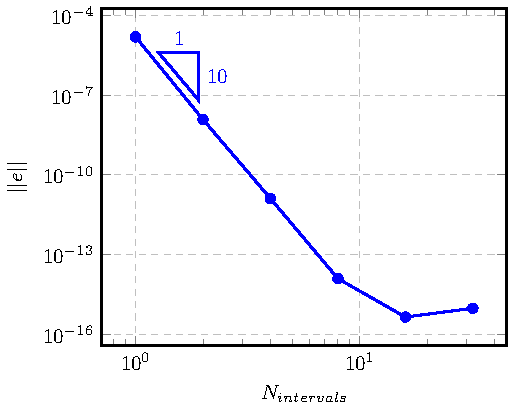
\includegraphics[scale=.90]{F1e0.pdf}}\hfill
    \subfloat[Function 1 $(\epsilon = 10^{-4})$ \label{fig:f1e4}]{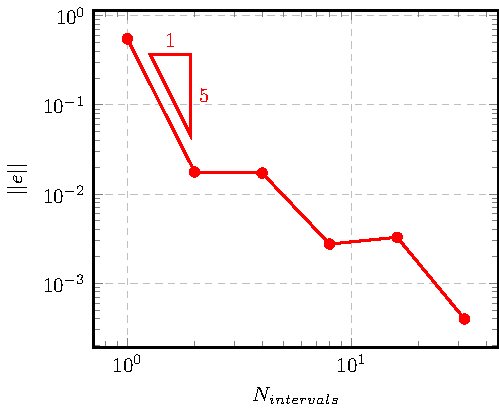
\includegraphics[scale=.90]{F1e4.pdf}} \vskip 5mm
    \subfloat[Function 2 \label{fig:f2}]{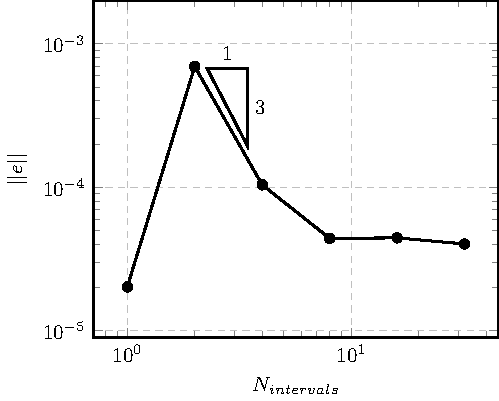
\includegraphics[scale=.90]{F2.pdf}} \hfill
    \subfloat[Function 3 \label{fig:f3}]{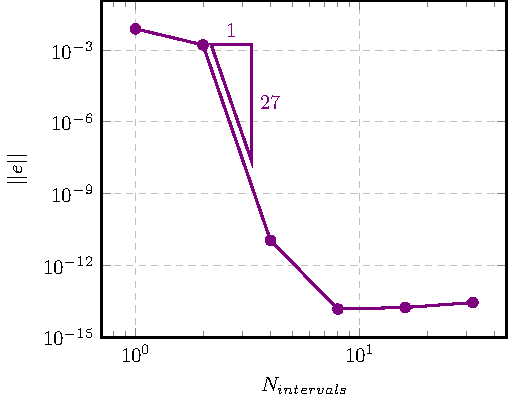
\includegraphics[scale=.90]{F3.pdf}}
    \caption{Convergence plots for the Gauss-Legendre Rule with four points.}
    \label{fig:gauss4_convergence}
\end{figure}
